\section{Resultados}
\label{sec:resultados}

\subsection{Búsqueda de hiperparámetros}
\label{sec:busqueda}

\begin{table}[t]
  \centering
  \caption{Búsqueda manual de hiperparámetros, solo en validación (\NVal{} imágenes). Cada fila
    cambia un único hiperparámetro de la referencia (tasa $10^{-3}$, lote de 64, cinco bloques de
    32 a 256 filtros, sin capa oculta, ReLU); todas usan la semilla 42. Pérdida: pérdida de
    validación en la mejor época. En negrita, la configuración elegida como modelo final.}
  \label{tab:busqueda}
  \small
  \setlength{\tabcolsep}{3.3pt}
  \TablaBusqueda
\end{table}

\begin{figure}[t]
  \centering
  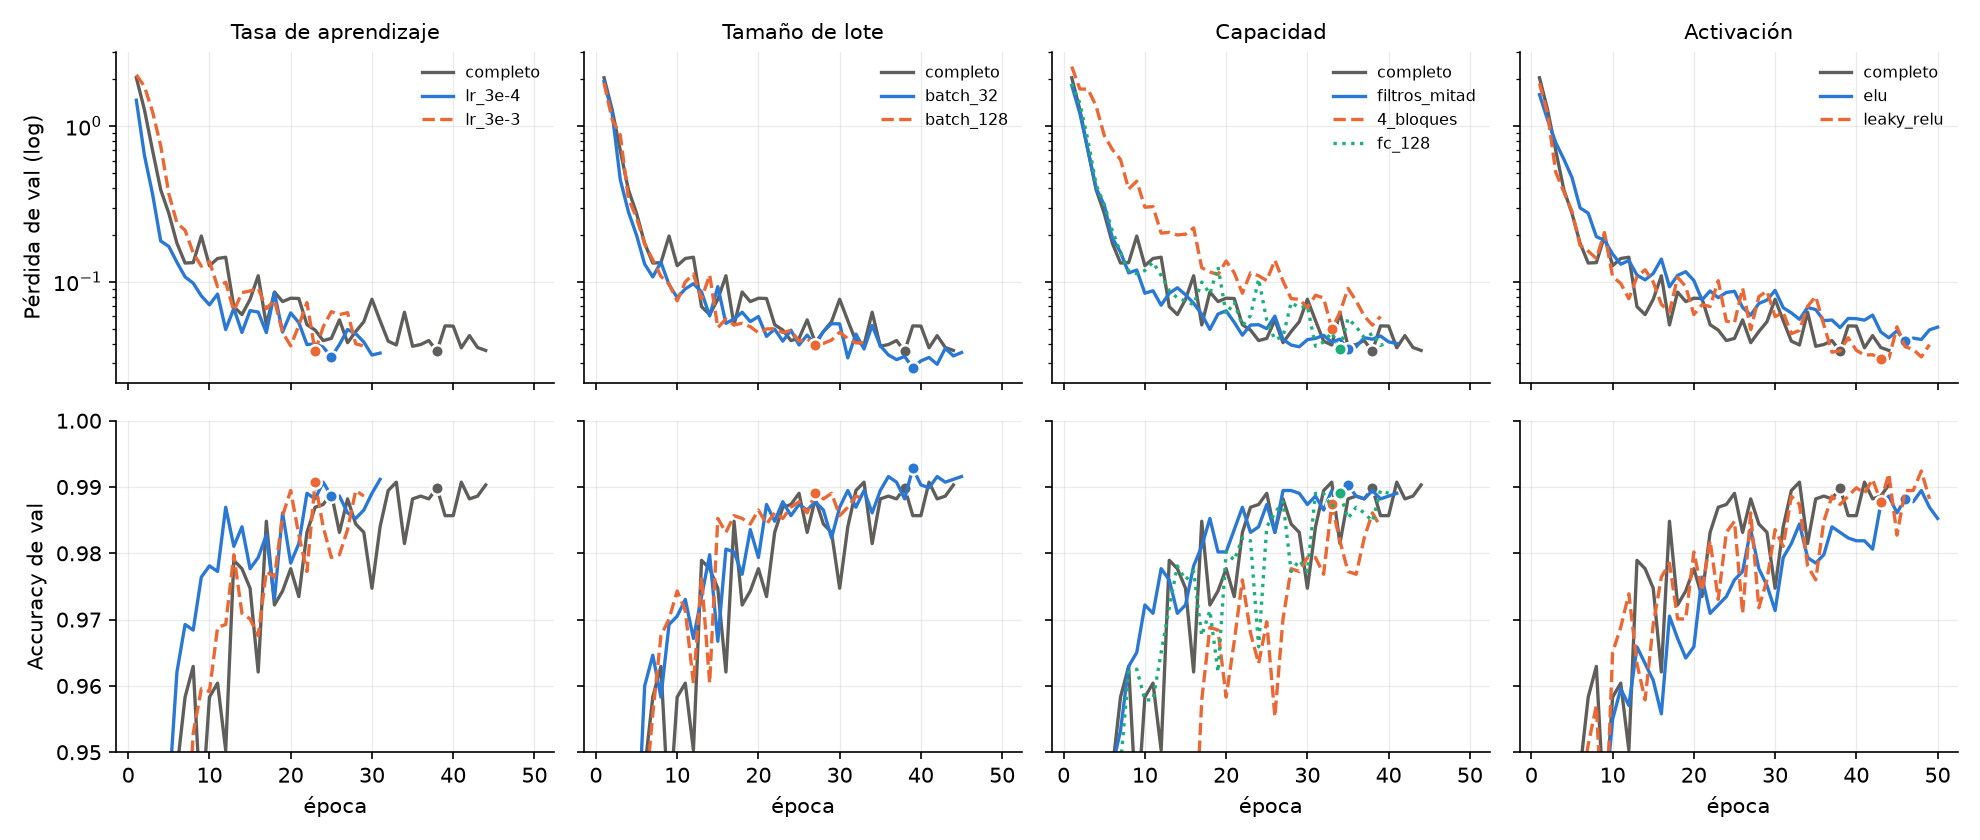
\includegraphics[width=\linewidth]{figures/busqueda_curvas.png}
  \caption{Curvas de validación de la búsqueda, un panel por tipo de hiperparámetro; en gris, la
    referencia. Arriba, la pérdida (escala logarítmica); abajo, la exactitud por encima del
    95\,\%. El punto marca la mejor época.}
  \label{fig:busqueda}
\end{figure}

La red es poco sensible a los cambios probados (\cref{tab:busqueda,fig:busqueda}): salvo el lote
de 32, todas las configuraciones quedan entre el \AccValBusquedaMin{} y el \AccValBusquedaMax{} de
exactitud de validación, a pocas imágenes de la referencia (\AccValCompleto). Para dar una medida
del ruido, dos ejecuciones idénticas del modelo completo con distinta semilla obtienen
\AccValCompleto{} y \AccValCompletoS. Con las tasas de $3\cdot10^{-3}$ y $3\cdot10^{-4}$ la parada
anticipada actúa antes (épocas \EpocasLrAlta{} y 31, frente a \EpocasCompleto), sin cambiar la
exactitud. Con la mitad de filtros la red rinde igual (\AccValFiltrosMitad) con cuatro veces menos
parámetros, lo que indica que está sobredimensionada. Quitar el último bloque es el cambio que más
empeora el resultado y el que más ralentiza el aprendizaje. La capa oculta no aporta nada, y ELU y
LeakyReLU quedan algo por debajo de ReLU.

El único cambio que mejora a la vez la exactitud y la pérdida de validación es el lote de 32
(\ErroresValFinal{} errores, frente a \ErroresValCompleto): con la misma tasa, da el doble de
actualizaciones por época y un gradiente más ruidoso, que actúa como regularizador. Según el
criterio fijado, pasa a ser el modelo final. Aun así, su ventaja procede de una sola ejecución y de
elegir la mejor de diez configuraciones, así que su exactitud de validación tiende a ser optimista.

\subsection{Modelo final}
\label{sec:test}

\begin{figure}[t]
  \centering
  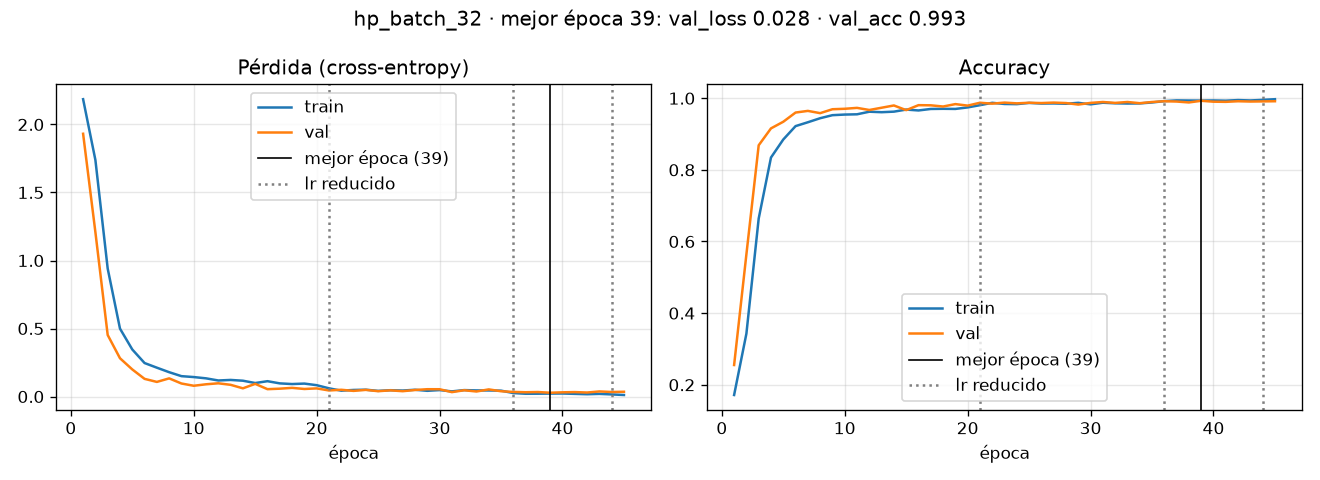
\includegraphics[width=0.92\linewidth]{final/curves.png}
  \caption{Pérdida y exactitud de entrenamiento y validación del modelo final (lotes de 32).
    Línea continua: mejor época (pesos restaurados); punteadas: reducciones de la tasa de
    aprendizaje.}
  \label{fig:curvas}
\end{figure}

La parada anticipada detuvo el entrenamiento en la época \EpocasFinal{} y restauró los pesos de
la \MejorepocaFinal{} (\cref{fig:curvas}). La exactitud de validación supera el 95\,\% en la
época \EpocanoventaycincoFinal, y las reducciones de la tasa (épocas \ReduccioneslrFinal) producen
las mejoras finales. Las curvas de entrenamiento y validación casi se superponen (diferencia
final: \BrechaFinal{} puntos), así que no hay sobreajuste apreciable. Al principio, la exactitud de
validación supera a la de entrenamiento porque esta se mide con el \emph{dropout} activo y sobre
imágenes aumentadas.

Evaluado una sola vez en test (\NTest{} imágenes de \PersonasTest{} personas), el modelo final
alcanza una exactitud del \AccTestFinal{} (IC del 95\,\%: \AccTestFinalIC) y una F1 macro del
\FoneTestFinal, con \ErroresTestFinal{} errores, unos 14 puntos por encima del objetivo. El modelo
completo, el final anterior, obtuvo un \AccTestCompleto{} (IC: \AccTestCompletoIC) con
\ErroresTestCompleto{} errores. Sobre las mismas imágenes, \SolofinalCompleto{} las acierta solo
el modelo final y \SolovarianteCompleto{} solo el completo (McNemar: \PmcnemarFinalCompleto). La
mejora de validación no se traslada al test, como cabe esperar si se debía en parte al ruido y a
la selección: la exactitud de validación del modelo final (\AccValFinal) supera a la de test,
mientras que en el completo coincidían. Ninguna de las conclusiones depende de cuál de los dos se
tome como final.

\begin{figure}[t]
  \centering
  \begin{minipage}[c]{0.575\linewidth}
    \centering\footnotesize
    \setlength{\tabcolsep}{1.8pt}
    \captionof{table}{Métricas por clase del modelo final en test.}
    \label{tab:porclase}
    \TablaPorClase
  \end{minipage}\hfill
  \begin{minipage}[c]{0.405\linewidth}
    \centering
    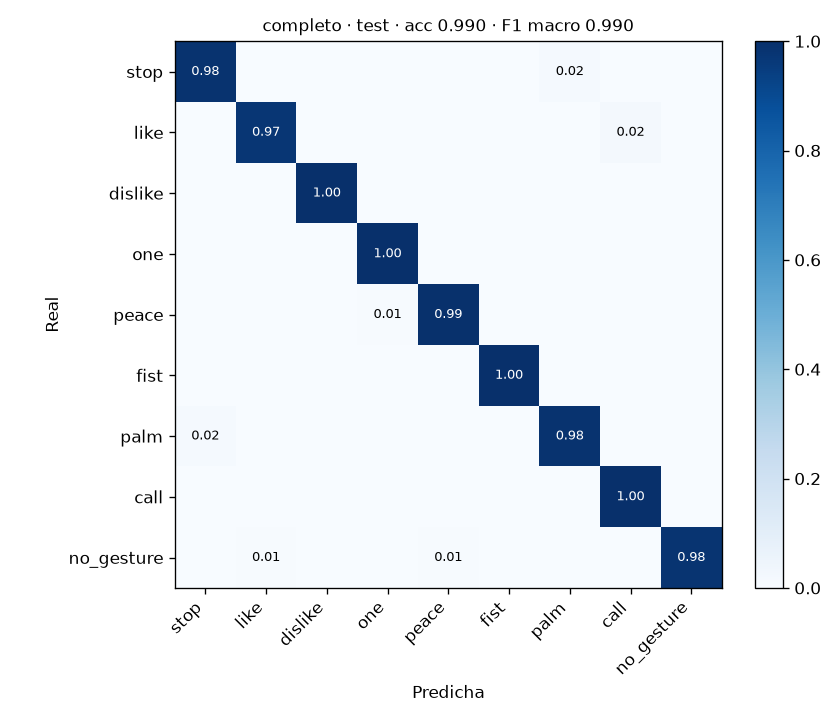
\includegraphics[width=\linewidth]{final/confusion_test.png}
    \captionof{figure}{Matriz de confusión del modelo final en test, normalizada por filas (la
      diagonal es el \emph{recall}).}
    \label{fig:confusion}
  \end{minipage}
\end{figure}

Todas las clases superan el 98\,\% de F1 (\cref{tab:porclase}); la peor es \PeorClaseTest{}
(\PeorFoneTest). Las confusiones más frecuentes (\cref{fig:confusion}) son
\ConfusionesTestFinal. \ErroresEnPares{} de los \ErroresTestFinal{} errores caen en dos pares de
gestos visualmente próximos: \cls{stop}/\cls{palm}, que solo se distinguen por si los dedos están
juntos o separados, y \cls{like}/\cls{call}, que se diferencian por el meñique. Para el robot, el
error más grave es tomar una mano en reposo por una orden: \FalsasActivaciones{} de los
\NNoGestureTest{} ejemplos de \cls{no\_gesture} de test (\TasaFalsasActivaciones) se clasificaron
como algún gesto.

\subsection{Estudio de ablación}
\label{sec:ablacion}

\begin{table}[t]
  \centering
  \caption{Ablación: media de las semillas 42 y 43. Cada variante quita un único componente del
    modelo completo (lotes de 64); la última columna da las épocas de cada semilla.
    $^\dagger$ResNet18 se entrenó una sola vez.}
  \label{tab:ablacion}
  \small
  \setlength{\tabcolsep}{4.5pt}
  \TablaAblacion
\end{table}

La normalización por lotes es la única ablación con un efecto claro (\cref{tab:ablacion}). Sin BN,
la exactitud media en test baja al \AccTestMediaSinBn, frente al \AccTestMediaCompleto, y los
errores se duplican. De las imágenes en las que solo acierta uno de los dos modelos,
\SolocompletoSinBn{} las acierta el completo y \SolovarianteSinBn{} la variante sin BN
(\PmcnemarSinBn). Sin BN el aprendizaje es además mucho más lento: tras la primera época la
exactitud de validación es del \AccepocaunoSinBn, y no supera el 95\,\% hasta la época
\EpocanoventaycincoSinBn{} (la \EpocanoventaycincoCompleto{} en el completo). Con ambas semillas
agotó las 50 épocas sin converger, así que el resultado debe leerse como «con el mismo presupuesto
de épocas».

Quitar el \emph{dropout} (\PmcnemarSinDropout) o el aumento de datos (\PmcnemarSinAug) no tiene
un efecto distinguible de la variación entre ejecuciones: dos ejecuciones idénticas del modelo
completo cometen \ErroresTestCompleto{} y \ErroresTestCompletoS{} errores en test. Su huella está
en la dinámica del entrenamiento. Sin aumento de datos, la red memoriza el conjunto de
entrenamiento, la diferencia entre entrenamiento y validación es la mayor de la ablación
(\BrechaSinAug{} puntos, frente a \BrechaCompleto) y la parada actúa antes (épocas
\EpocasSinAug{} y \EpocasSinAugS).

\subsection{Comparación con ResNet18 y coste}
\label{sec:resnet}

ResNet18 preentrenado alcanza un \AccepocaunoResnet{} de exactitud de validación tras la primera
época (GestureCNN: \AccepocaunoFinal). En test obtiene un \AccTestResnet{} (IC:
\AccTestResnetIC), con \ErroresTestResnet{} errores frente a los \ErroresTestFinal{} de
GestureCNN. La diferencia no es significativa: \SolovarianteResnet{} imágenes las acierta solo
ResNet18 y \SolofinalResnet{} solo GestureCNN (\PmcnemarFinalResnet). El preentrenamiento acelera
la convergencia, pero no podemos afirmar que un modelo con \RatioParams{} veces más parámetros
generalice mejor.

En cuanto al coste, el número de parámetros engaña. GestureCNN tiene \RatioParams{} veces menos
parámetros que ResNet18, pero hace \RatioMacs{} veces más operaciones por imagen (\MacsFinal{}
frente a \MacsResnet{} MACs), porque sus dos primeros bloques trabajan a $128^2$ y $64^2$\,px y
acumulan el \FracMacsPrimerosBloques{} de las operaciones. Aun así, con una sola imagen clasifica
un recorte en \LatCpuFinal{} en la CPU (\CPU) y en \LatCudaFinal{} en la GPU, frente a
\LatCpuResnet{} y \LatCudaResnet{} de ResNet18. Los dos modelos caben holgadamente en los 33\,ms
por fotograma de una cámara a 30\,fps.

\subsection{Explicabilidad con Grad-CAM}
\label{sec:gradcam}

En los aciertos de validación, la activación se concentra sobre la mano, no sobre el fondo ni la
cara, y señala los rasgos de cada gesto: en \cls{call}, por ejemplo, el mapa tiene dos máximos,
sobre el pulgar y sobre el meñique. La \cref{fig:gradcam} muestra los errores más seguros, que son
de tres tipos:
\begin{itemize}
  \item \textbf{Ruido de etiqueta}: un \cls{no\_gesture} que es, de hecho, una palma abierta, y
    que la red clasifica como \cls{palm} con probabilidad 1,00.
  \item \textbf{Objetos con forma de gesto}: un teléfono, o el borde vertical de un mueble junto
    al índice, que la red lee como los dedos de \cls{peace}.
  \item \textbf{Pares próximos o imágenes de baja calidad}: \cls{palm}$\to$\cls{stop} con una
    separación intermedia entre los dedos, \cls{like} de perfil confundidos con \cls{call} o
    \cls{one}, y un \cls{palm} pixelado.
\end{itemize}
En los pares próximos, los mapas de la clase real y de la predicha coinciden: la red mira el lugar
correcto, pero la evidencia es ambigua.

\begin{figure}[t]
  \centering
  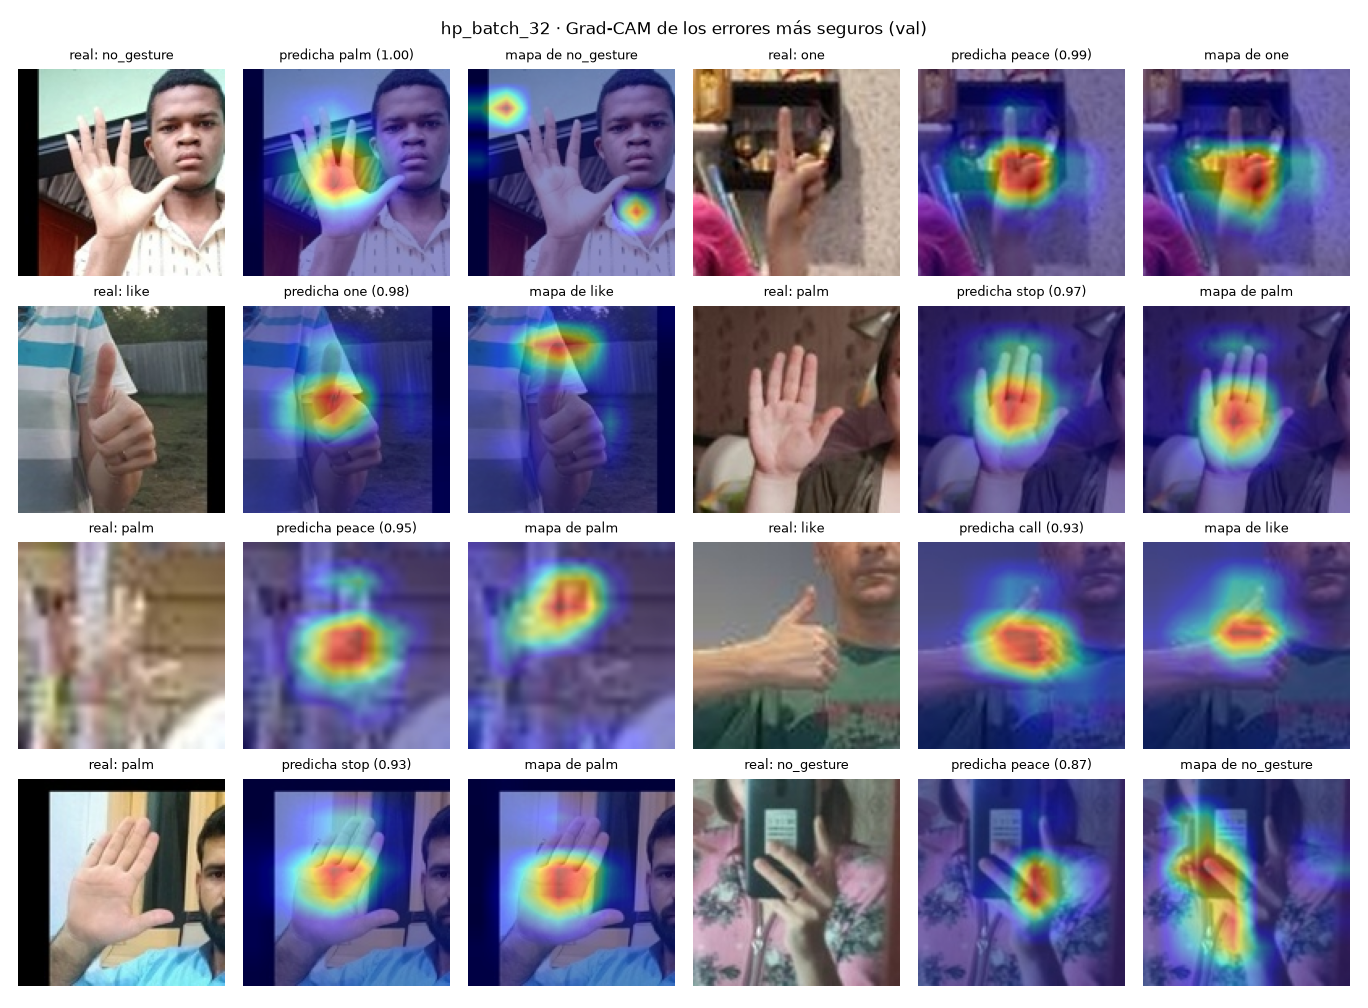
\includegraphics[width=0.85\linewidth]{final/gradcam_errores_val.png}
  \caption{Errores más seguros del modelo final en validación. Para cada uno: la imagen con su
    clase real, el mapa de la clase predicha y el de la clase real.}
  \label{fig:gradcam}
\end{figure}
